\documentclass{article}
\usepackage{hyperref,listings,graphicx,xcolor,asmath,lmodern}

\title{Google Earth Engine Integration with Open Data Cube}
\author{Andrew Lubawy\\ Analytical Mechanics Associates}
\date{September 2020}

\begin{document}
\maketitle
\tableofcontents

\part{Prerequisites}
\chapter{Setup Google API for Google Earth Engine}
The first step is to setup the API to use the
\href{https://developers.google.com/earth-engine/reference}{Google Earth Engine
REST API}. To do
this you need to create a project here:
\url{https://console.cloud.google.com/}. Go to the
\href{https://console.cloud.google.com/apis/dashboard}{API \& Services
Dashboard}
from the developer console.

\begin{figure}
	\caption{Create credentials}
	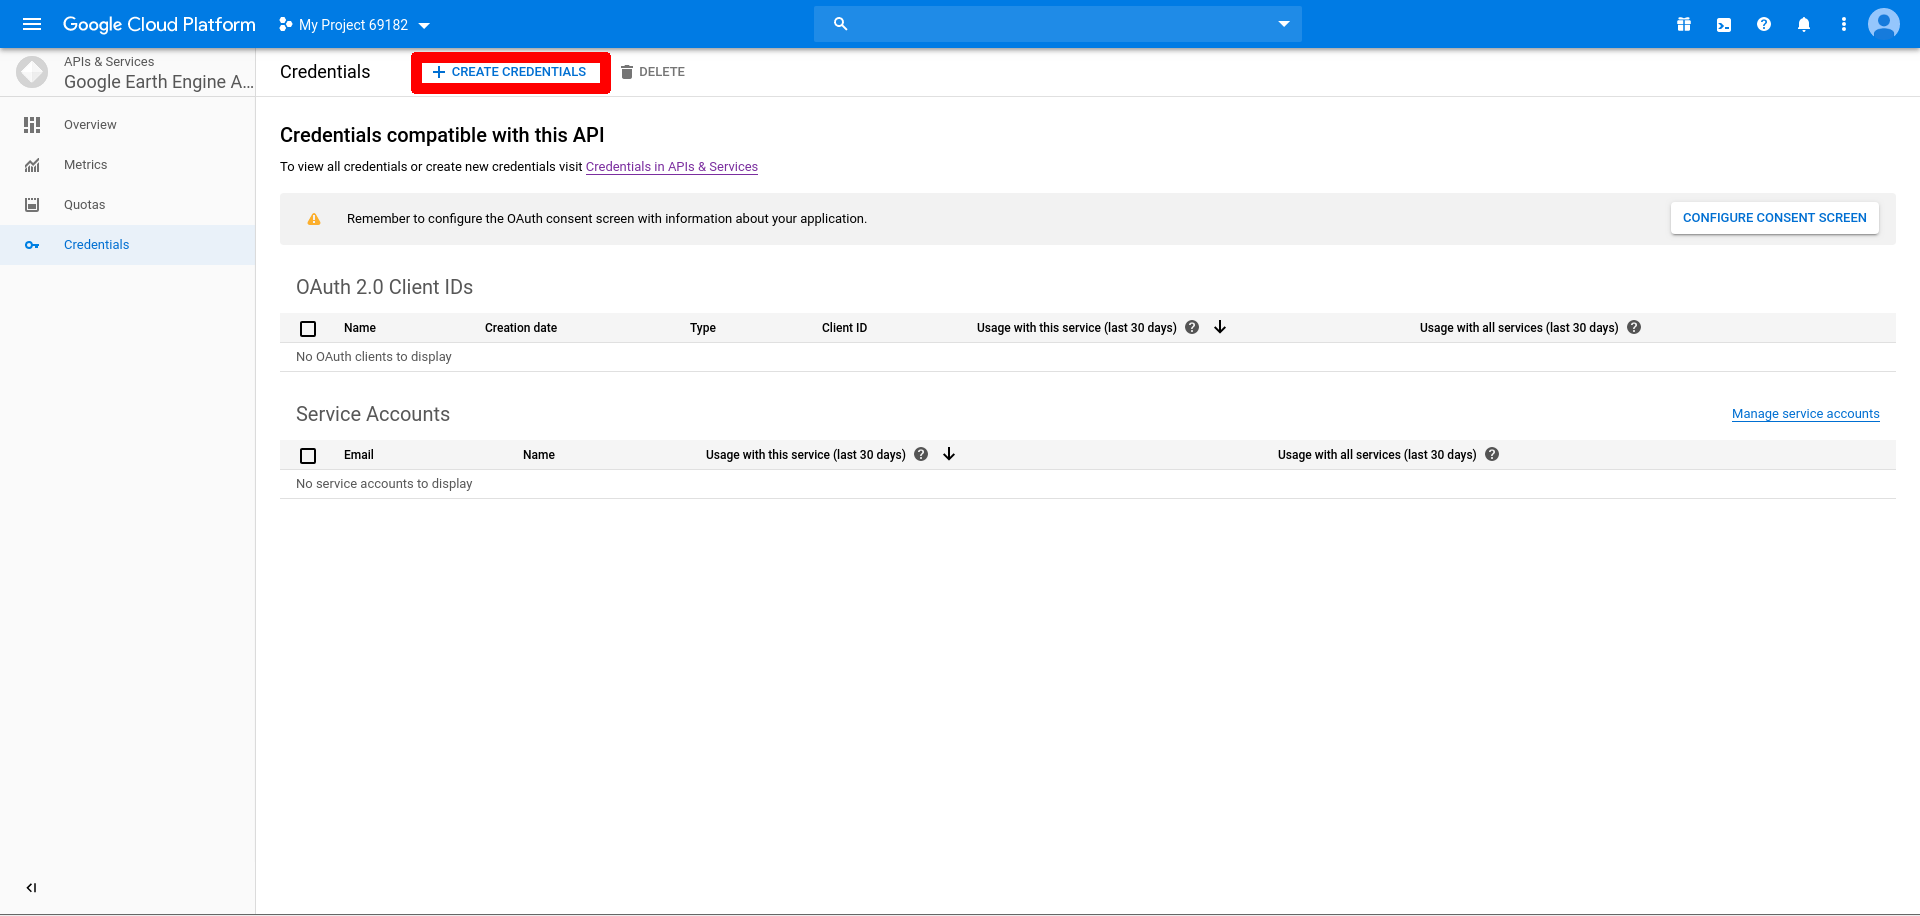
\includegraphics{images/image1.png}
\end{figure}

Select the button in the red box according to Figure 1. This will pull up the
API library. Search for Earth Engine, select it, and then enable it for the
project.

The next step to setup the API is to create a Service Account. To do this
navigate to the
\href{https://console.cloud.google.com/apis/api/earthengine.googleapis.com/credentials}{API
\& Services Credentials} page for the API.

\begin{figure}
	\caption{Enabling APIs and services}
	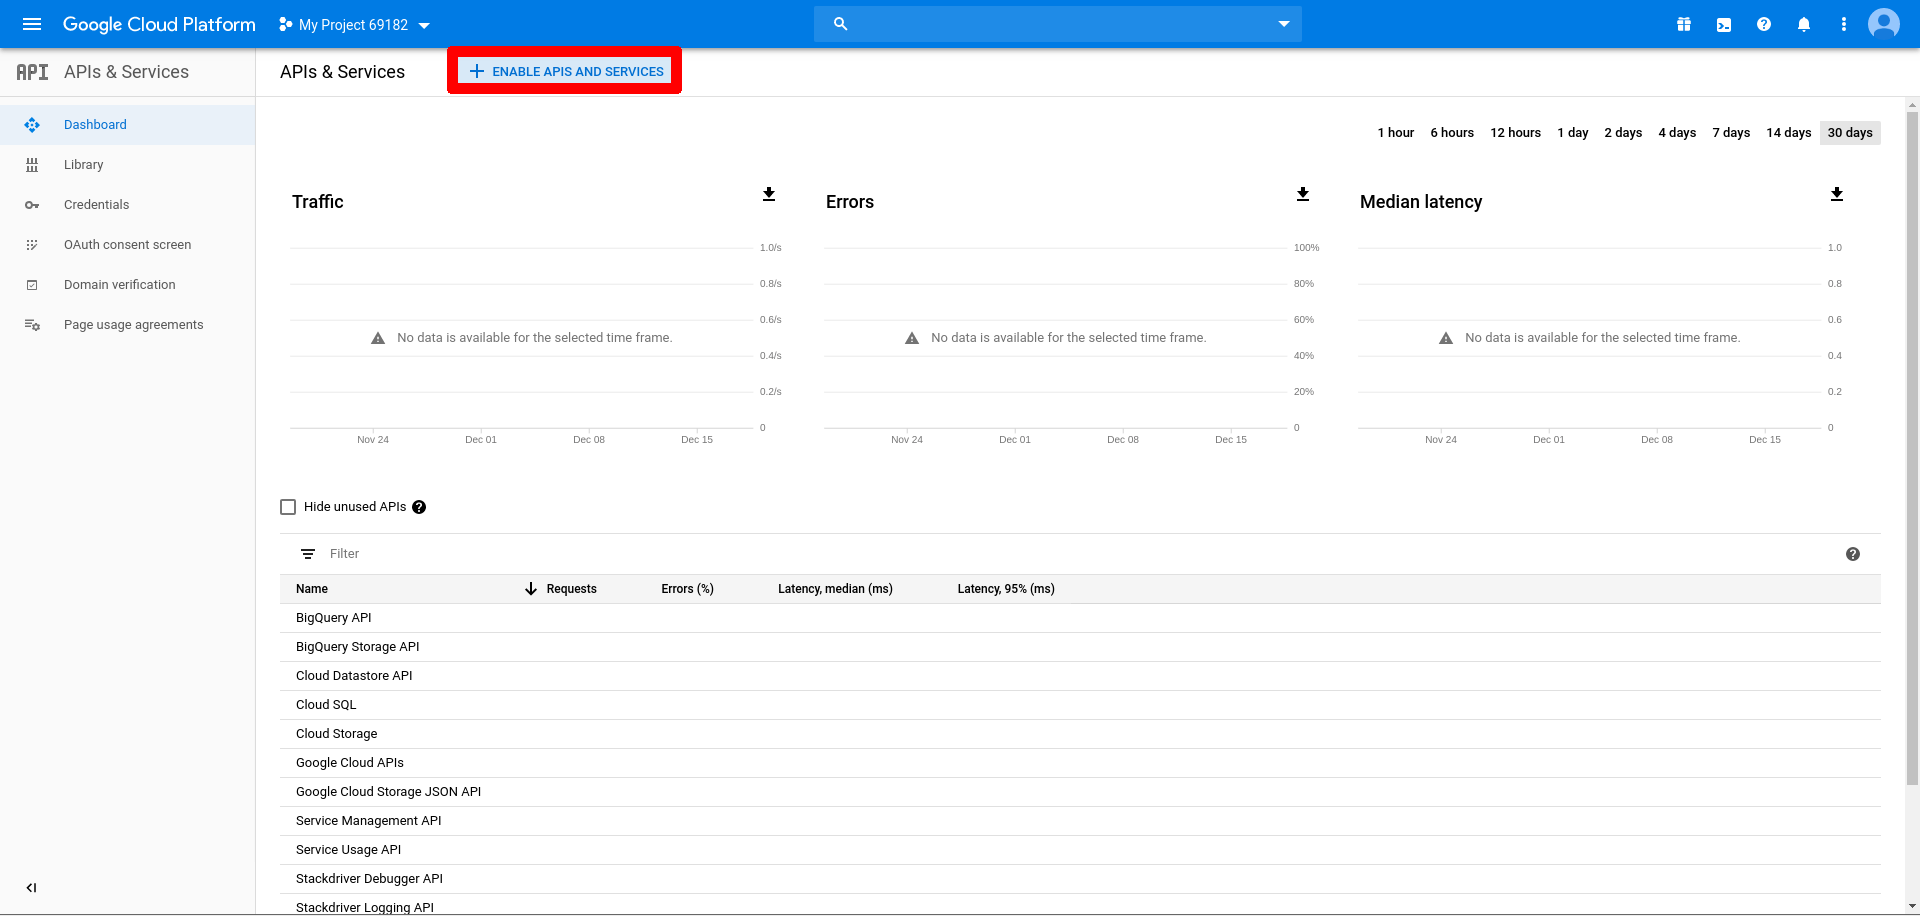
\includegraphics{images/image2.png}
\end{figure}

Click the button in the red box for Figure 2 and select Service Account. Fill
out the form
and click next. You will likely need to add Owner roles in the next section.
Click the Role selection box, type Owner in the filter field, and then select
the Owner choice to add it as the Role. Click next. In this section click add
key and select the JSON option. This will download a JSON file with your key’s
credentials for the Service Account. \textbf{Keep this file secure and don’t
lose it.} This file will act as the API key for accessing GEE data. Once
you’ve got the file, click done.

This last step is only necessary if the GEE REST API is still unreleased to the
public and if you have the proper permissions to do so. If those conditions are
met then you will have to email a Google employee your Service Account email as
indicated by the red box from the
\href{https://console.cloud.google.com/apis/api/earthengine.googleapis.com/credentials}{API
\& Services Credentials} page in Figure 3.

\begin{figure}
	\caption{Service account email}
	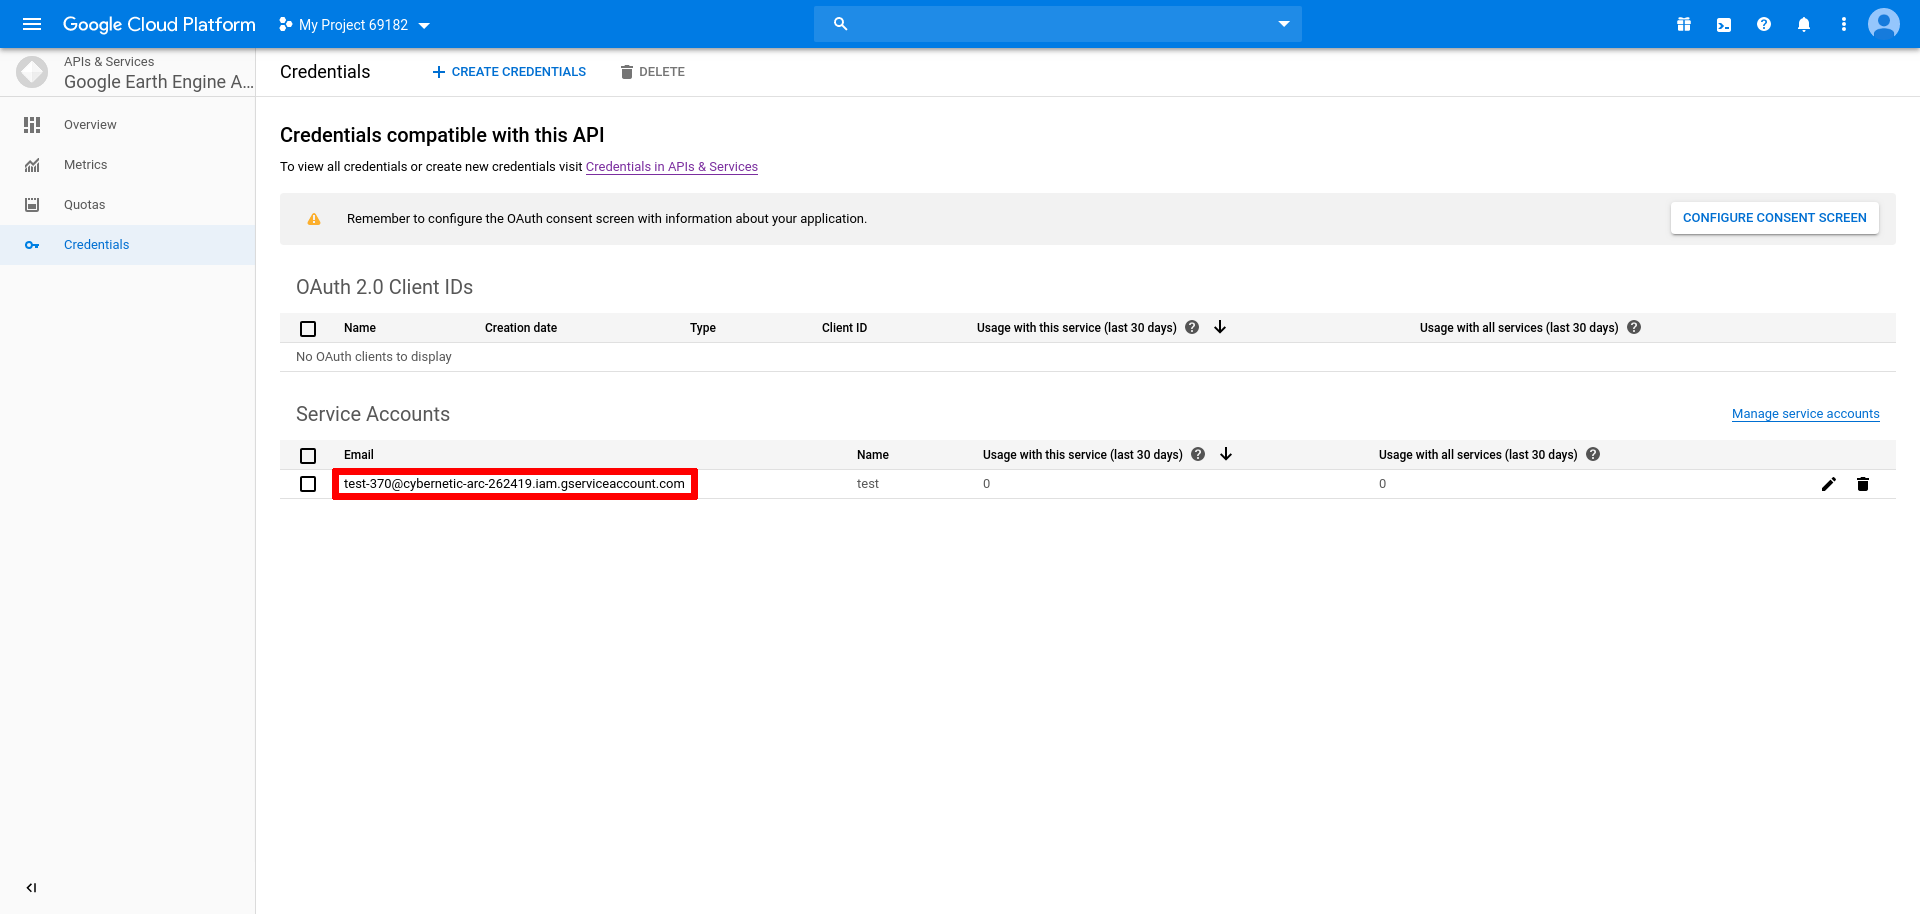
\includegraphics{images/image3.png}
\end{figure}

\part{ODC with GEE Usage}
\chapter{Installing ODC}
Setup is simple and straightforward. You can follow one of the installation
instructions here:
\url{https://datacube-core.readthedocs.io/en/latest/ops/install.html}. Our
preferred method is to setup a Python virtualenv and use
\lstinline{pip install datacube} and some extra packages
\lstinline{pip install jupyter matplotlib scipy}. More suggested packages can
be found in the CEOS SEO
\href{https://github.com/ceos-seo/data_cube_utilities}{GitHub repository for
Jupyter notebook utilities}.

The other option is to have ODC install datacube with the odc-gee package which
includes it as a required dependency.

\chapter{Indexing Data}
Indexing data is nearly identical to
\href{https://datacube-core.readthedocs.io/en/latest/ops/indexing.html}{normal
ODC indexing} and makes heavy use of modified
\href{https://github.com/opendatacube/datacube-dataset-config/blob/master/scripts/index_from_s3_bucket.py}{AWS
S3 indexing scripts}. It also uses the following Python packages:
\begin{itemize}
	\item google-api-python-client
	\item google-auth
	\item google-auth-oauthlib
\end{itemize}
These packages make it easy to authenticate and connect with the GEE API. This
will allow for using the API to retrieve metadata on products to be indexed.

The first step to indexing is to create a product definition. This
process can be found in the ODC documentation:
\url{https://datacube-core.readthedocs.io/en/latest/ops/product.html}. The
primary goal is to define the most relevant and basic information about a
\href{https://developers.google.com/earth-engine/datasets}{GEE catalog entry}.
If using the odc-gee package, it is important to make sure aliases are included
in the measurements field with an alias in the list being the defined
band in the GEE catalog. For example, the blue band in a Sentinel-2 product
will have "B2" as an alias. This is to allow products to change names
while retaining the mapping to the band name as defined by the API. It also
performs a check to make sure a dataset has all the required bands to prevent a
failure to index. Sentinel-1 is an example of this where it will rarely exclude
the typical "VV" and "VH" bands for "HH" and "HV" instead. ODC needs all bands
defined in the product specification to be present. The odc-gee also includes a
script to guide the process. This can be ran by running
\lstinline{new_product <product-name>.yaml}.

An example of a Sentinel-1 product definition for Google Earth Engine (note:
single precision float32 was chosen over original data's double precision
float64 to conserve memory on load):
\begin{lstlisting}[language=json]
name: s1_google
description: Sentinel-1A/B SAR sigma0 scenes, processed by Google - Apply orbit
file, GRD border noise removal, thermal noise removal, radiometric calibration,
and terrain correction (SRTM 30m DEM).
metadata_type: eo

metadata:
	format: {name: GeoTIFF}
	instrument: {name: SAR}
	platform: {code: SENTINEL-1}
	product_type: GRD

storage:
	crs: EPSG:4326
	resolution:
		longitude: 0.0000898311175
		latitude: -0.0000898311175

measurements:
	- name: vh
	  aliases: [VH]
	  dtype: float32
	  nodata: 0
	  units: 'DN'

	- name: vv
	  aliases: [VV]
	  dtype: float32
	  nodata: 0
	  units: 'DN'
\end{lstlisting}

The next step is to create a dataset configuration file. This requires
a little more effort than just following the
\href{https://datacube-core.readthedocs.io/en/latest/ops/dataset_documents.html}{ODC
guide} for datasets, but it should still be a simple process. The S3 script
linked earlier is modified and used here with the ODC guide as a blueprint for
doing the same for GEE data. Instead of grabbing the metadata from an AWS S3
bucket, the data will be retrieved through the API libraries linked above. This
will need the service account credentials downloaded in the prerequisites
section.

The major difference between the S3 and GEE indexing will be in the band path
format. GEE indexed data is accessed by using rasterio
which wraps GDAL which smartly picks a driver for
\href{https://gdal.org/drivers/raster/eedai.html}{pulling from the GEE API}.
Therefore the band path will need to be in a format that GDAL will recognize
and which the API driver will use: \lstinline{EEDAI:[asset][:band_names]}.

An example of a Sentinel-1 band path for GEE in ODC broken up into its various
parts:
\begin{lstlisting}[language=python]
'EEDAI:' + 'projects/earthengine-public/assets/' +
'COPERNICUS/S1_GRD/S1A_IW_GRDH_1SDV_20160121T181002_20160121T181027_009596_00DF74_ABC5'
+ ':VV'
\end{lstlisting}

Currently, this entire process has been turned into various Python modules, and
on top of those is now a script which can do this process in a more automated
fashion. This is in the odc-gee package and can be used like so for a specified
Sentinel-1 product:
\lstinline{index_gee --asset COPERNICUS/S1_GRD --product s1_google}. This will
iterate through every available image in the GEE catalog entry for its entire
time extent. It will then attempt to parse the image's metadata into a dataset
document to add to the ODC index. Other options are available for specifying
regions or allowing updates in the index.

\section{How the API is Parsed}
The script uses the
\href{https://developers.google.com/earth-engine/reference}{GEE REST API}. It
specifically queries the
\href{https://developers.google.com/earth-engine/reference/rest/v1alpha/projects.assets/listImages}{\lstinline{listImages}
endpoint} to receive a list of datasets. Then it will iterate over the results
and parse the available metadata into a format for an ODC dataset document:
\url{https://datacube-core.readthedocs.io/en/latest/ops/dataset_documents.html}
(currently using the deprecated EO format). The dataset document is constructed
using what was defined in the product definition as well as what is provided by
the metadata from the API result.
\end{document}
